\section{Methods}\label{sec:methods}

This section will detail the implementation and necessary technological foundation, for applying the theories described,
in order to produce the experimental results for answering the research question. The section will also detail the necessary information,
for reproducing and understading the experimental results and their becoming.

\subsection{Experimental Setup}\label{subsec:setup}
The experimental setup are comprised of the following components:
\begin{itemize}
    \item Dataset
    \item Model
    \item Training- and Validation-Loop
    \item Test loop
\end{itemize}

These four components all together make up the main functionality of the experiment, and will be detailed individually
below. The detailing will have its focus on how concepts and theories previously explained,
are formatted and shaped, in order to be viable for practical modelling purposes.

\subsection{Dataset}\label{subsec:dataset}
The data set is comprised of one row for each node for 695 molecules, with a the following fields for each node:
\begin{itemize}
    \item Atom-type
    \item Overall binding energy (target property)
    \item x-coordinate
    \item y-coordinate
    \item z-coordinate
    \item Graph id
\end{itemize}
The atom type signifies the type of atom for a given node by name. The overall binding energy is the target property, for the full catalyst
process. This means all nodes with identical graph id will have a identical overall binding energy. The x, y, and z coordinates are the coordinates
of the nodes in the molecular graph, measured in Ångstrøm.

These fields are then translated to the relevant datastructures, via the graph data set constructor. This constructor
defines the following data structures, for utilization in the modelling task. Important to say is that the data set constructor,
constructs a data set of popentially several graphs, and not only one. The data set consists of the following critical fields:
\begin{itemize}
    \item num\_nodes: Number of nodes in the data set of graphs
    \item node\_from: The node from which the edge originates
    \item node\_to: The node to which the edge points
    \item num\_graphs: Number of graphs in the data set
    \item node\_graph\_index: The index of the graph the edge resides in
    \item unique\_atoms: The number of unique atoms in the data set
    \item edge\_lengths: The lengths of the edges
    \item edge\_vector\_diffs: The vector differences of the edges
\end{itemize}

The number of nodes in dataset, allows for the model to create initial state representation structures with proper dimensions for the
modelling task. The node\_from property, allows for summation of all neighbouring node state representations, within the cutoff limit,
into the designated node, we are trying to model in the message block. The node\_to property, allows for initialising the state representation
of the node in the update block, namely the scalar properties and the vector properties. The scalar properties are concatenated tensors of
embedded atom representations, linked by the index in the node\_to property. For scalar properties it is zero-vectors, instead of embedded
tensors. The num\_graphs property is used to initalize the initial state representation of the graphs. The node\_graph\_index property
is an index linking an edge, to a corresponding graph. When summing over all neighbour nodes occur, the full message state representation of all
neighbours under the cutoff, is summed over the node\_graph\_index property, to produce a state representation of graphs. The unique\_atoms
property, allows for the embedding function to create a unique atom representation for each type of atom in the data set. The edge\_lengths
allow for a masking of the edges and thereby nodes that are not within the cutoff limit. The edge\_vector\_diffs are the vector differences
of the edges, being an input variable in the message block.



\subsection{Model}\label{subsec:model}

The model architecture consists of two main components, namely the Message block, and the Update block as formerly introduced in the
the theory section \ref{eq:message_block}, and \ref{eq:update_block}.  The Message block is conceptually responsible
for the message passing between the nodes in the graph, allowing for the flow of information between the nodes.
This information is then summed up and stored in state variables in the form of a scalar and vector representation.
This summation is done in a residual manner, following the implementation of the PAINN architecture\cite{PAINN}. An equation
defining the residual calculation of the scalar-properties\ref{eq:residual_scalar} and vector-properties\ref{eq:residual_vector}
can be found below, as well as an illustration of the message block\ref{img:message_block}.

\begin{equation}\label{eq:residual_scalar}
    \Delta \mathbf{s}_{i}^{m}= (\phi_{s}(\mathbf{s}) * \mathcal{W}_{s})_{i} = \sum_{j} \phi_{s}(\mathbf{s}) \circ \mathcal{W}_{s} \left ( \left \| r_{ij} \right \| \right )
\end{equation}

\begin{equation}\label{eq:residual_vector}
    \Delta \vec{\mathbf{v}}_{i}^{m}= \sum_{j} \vec{\mathbf{v}}_{j} \circ \phi_{vv}(\mathbf{s}_{j}) \circ \mathcal{W}_{vv} \left ( \left \| r_{ij} \right \| \right ) + \sum_{j} \phi_{vs}(\mathbf{s}_{j}) \circ \mathcal{W}'_{vs} \left ( \left \| r_{ij} \right \| \right ) * \frac{r_{ij}}{\left \| r_{ij} \right \|}
\end{equation}

\begin{figure}[H]
    \caption{Message Block}
    \centering\label{img:message_block}
    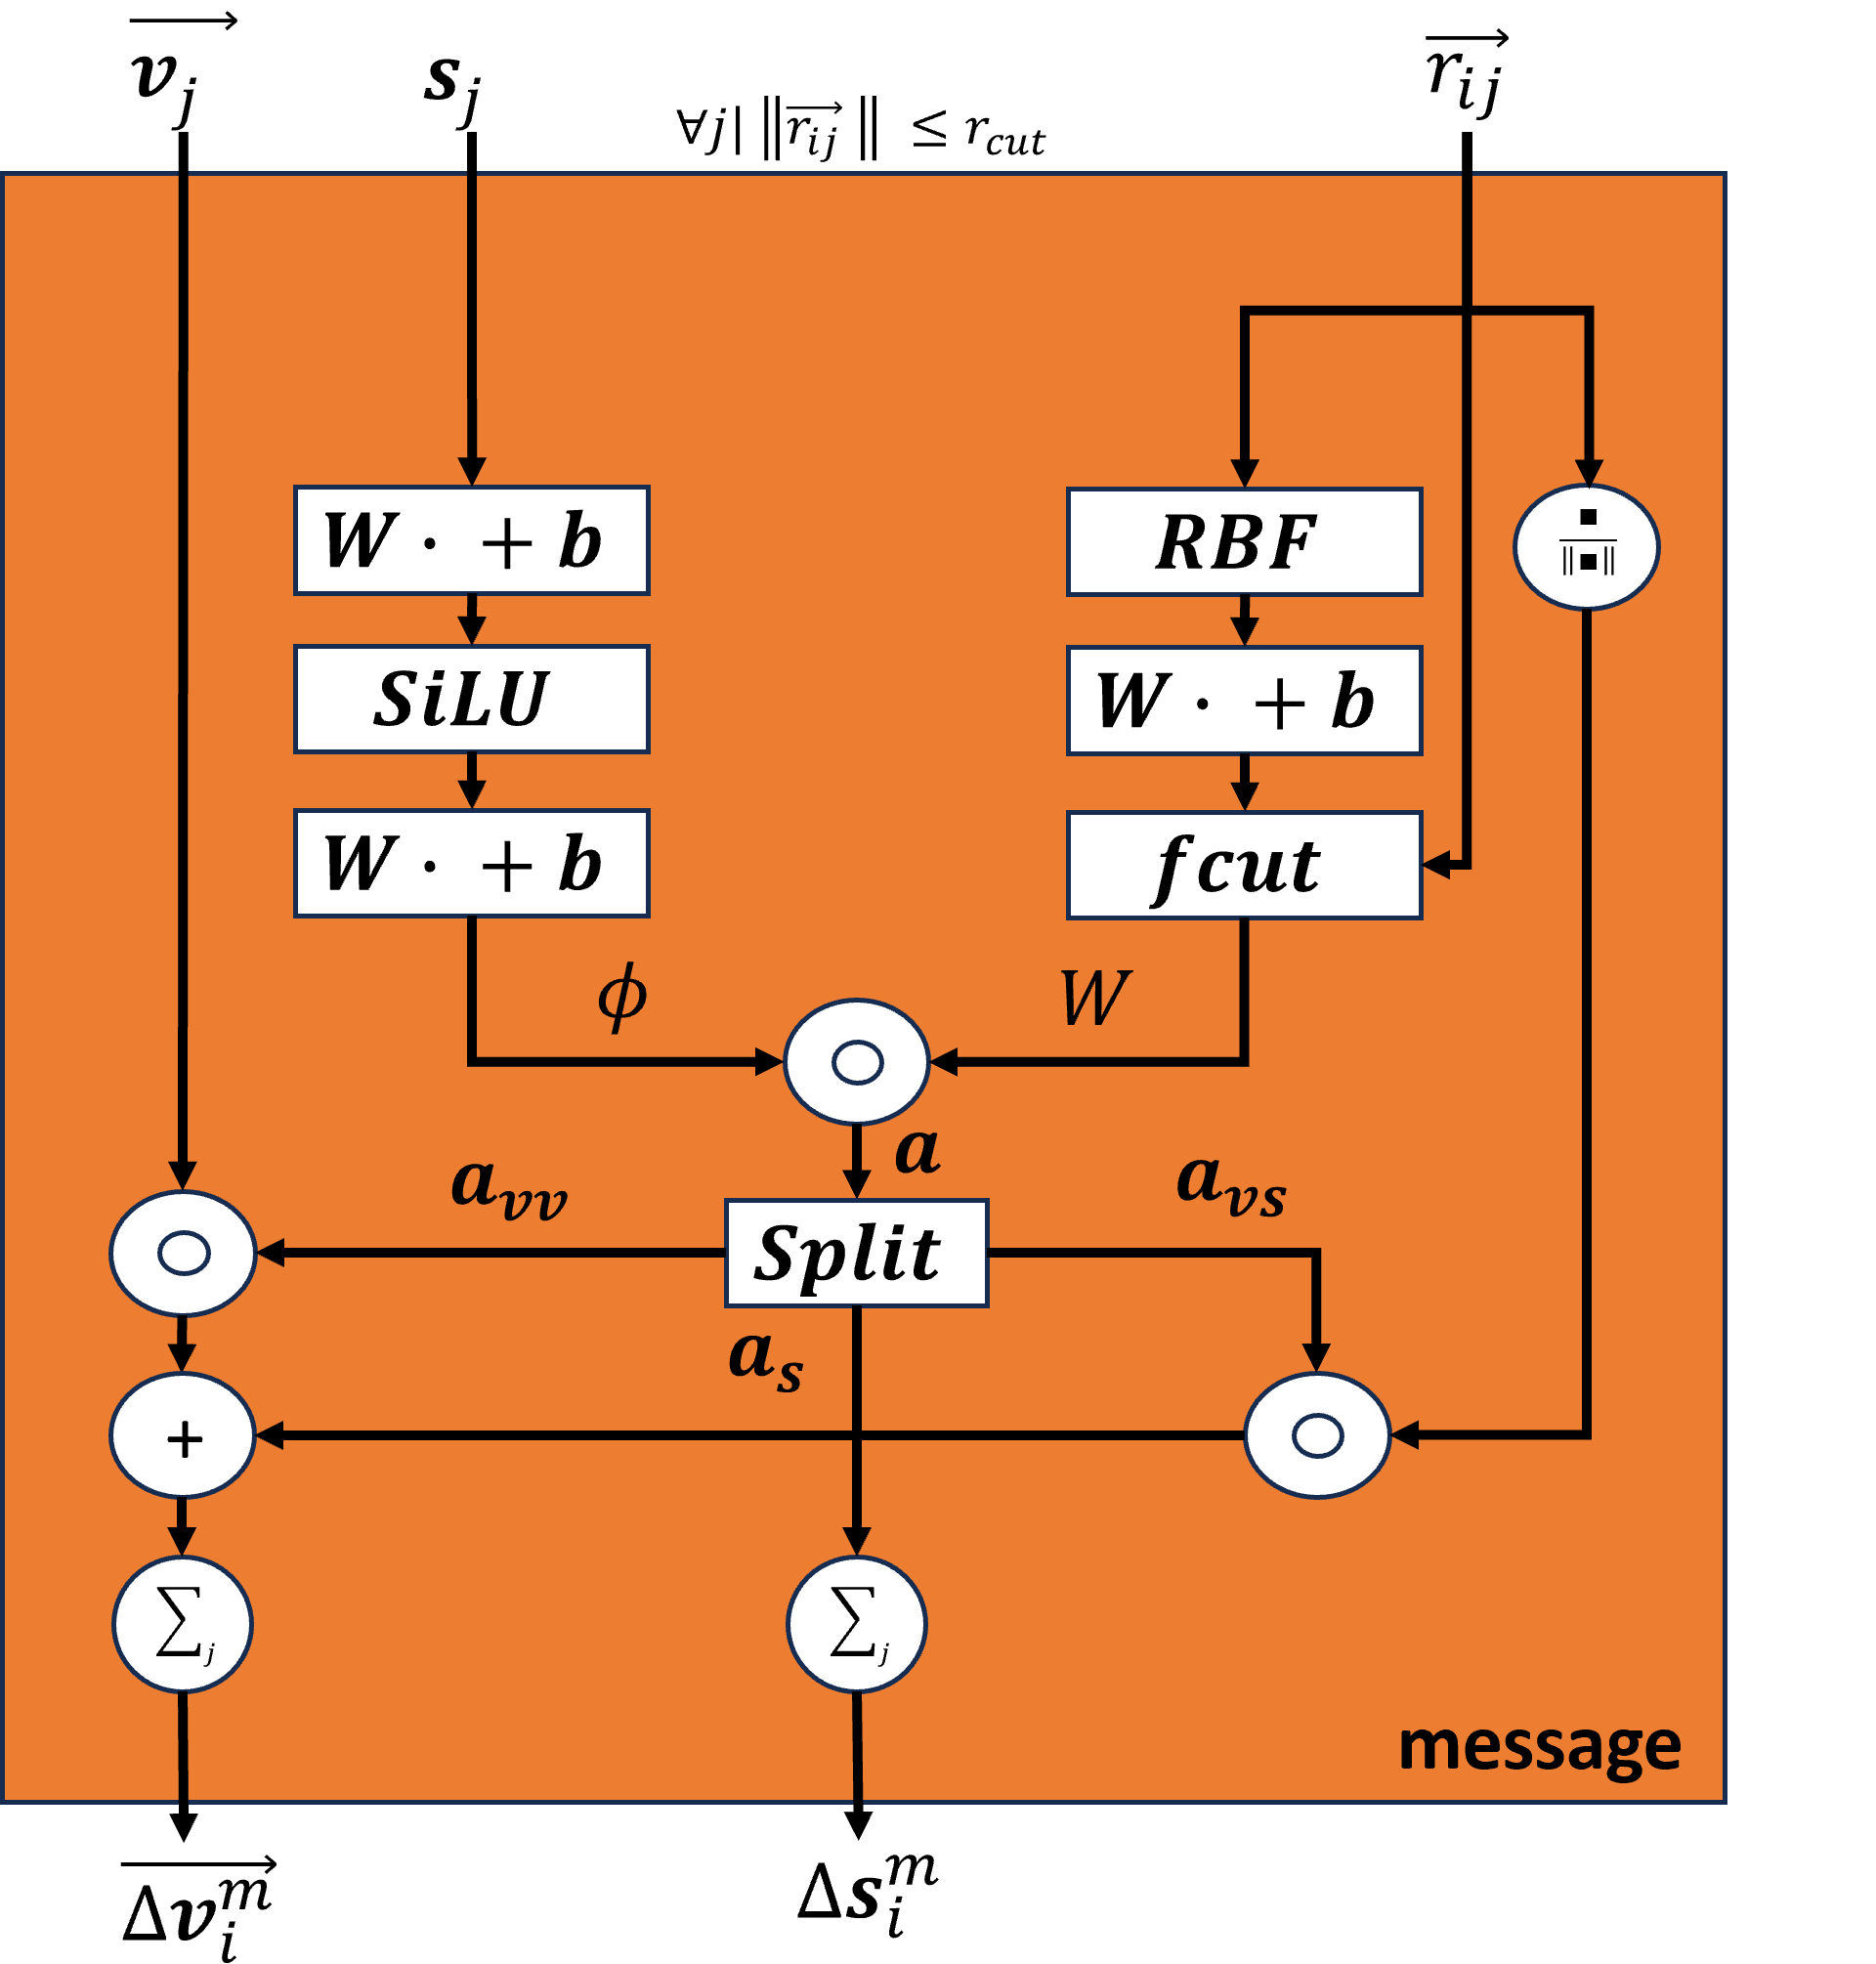
\includegraphics[width=250pt]{Images/Method/message_block.png}
\end{figure}

Worth noting about the figure, compared to the similar one in \cite{PAINN}, is the use of the \textit{r\_ij} vector, that also flow into
the 'fcut' function, as mentioned in \ref{subsec:modelling_task}. The model in this paper, does not highlight the dimension expansions
or collisions from network element to network element, due to the model parameters varying in size, as it is the scope of this project
to investigate similarities or dissimilarities in performance, with respect to the PAINN architecture and dissimilar state representation
sizes. both sizes $\phi$ and $\mathcal{W}$ are chosen sub-architectures based on the PAINN architecture from\cite{PAINN}. The image
also contains hints of the $\mathbf{a}$-tensor, which is a product of the $\phi$ and $\mathcal{W}$ tensors, and not highlighted in \cite{PAINN}.

The residual values produced in the message block, then used in the update block, in order to update the node states,
based on the summation over neighbouring states.
This structure is also heavily inspired by the PAINN architecture\cite{PAINN}. The below equations represent the residual updates
on both the scalar- \ref{eq:residual_scalar_update} and the vector- \ref{eq:residual_vector_update} properties. Below is also
a figure representing the update block\ref{img:update_block}.

\begin{equation}\label{eq:residual_scalar_update}
    \Delta \mathbf{s}_{i}^{u}= \mathbf{a}_{ss} \left ( \mathbf{s}_{i}, \left | \mathbf{V\vec{v}_{i}} \right | \right ) + \mathbf{a}_{sv} \left ( \mathbf{s}_{i}, \left | \mathbf{V\vec{v}_{i}} \right | \right ) \left \langle \mathbf{U\vec{v}_{i}}, \mathbf{V \vec{v}_{i}} \right \rangle
\end{equation}

\begin{equation}\label{eq:residual_vector_update}
    \Delta \mathbf{v}_{i}^{u}= \mathbf{a}_{vv} \left ( \mathbf{s}_{i}, \left | \mathbf{V\vec{v}_{i}} \right | \right ) \mathbf{U\vec{v}_{i}}
\end{equation}



The blocks are stacked in coupled sequences of five full rounds, like the illustration below highlights\ref{img:MPNN_arc}, a corresponsding model can be found
in \cite{PAINN}. The illustration shows an architecture comprised of three sets of message- and update-blocks, the implementation in this project utilized
five sets. The model representation property $\vec{v_i^{0}}$ is initialized to the zero vector, and the scalar property $S_{i}^{0}$
is initialized to a random embedding on atom level, for each node in the graph.


\begin{figure}[H]
    \caption{MPNN Full Architecture}
    \centering\label{img:MPNN_arc}
    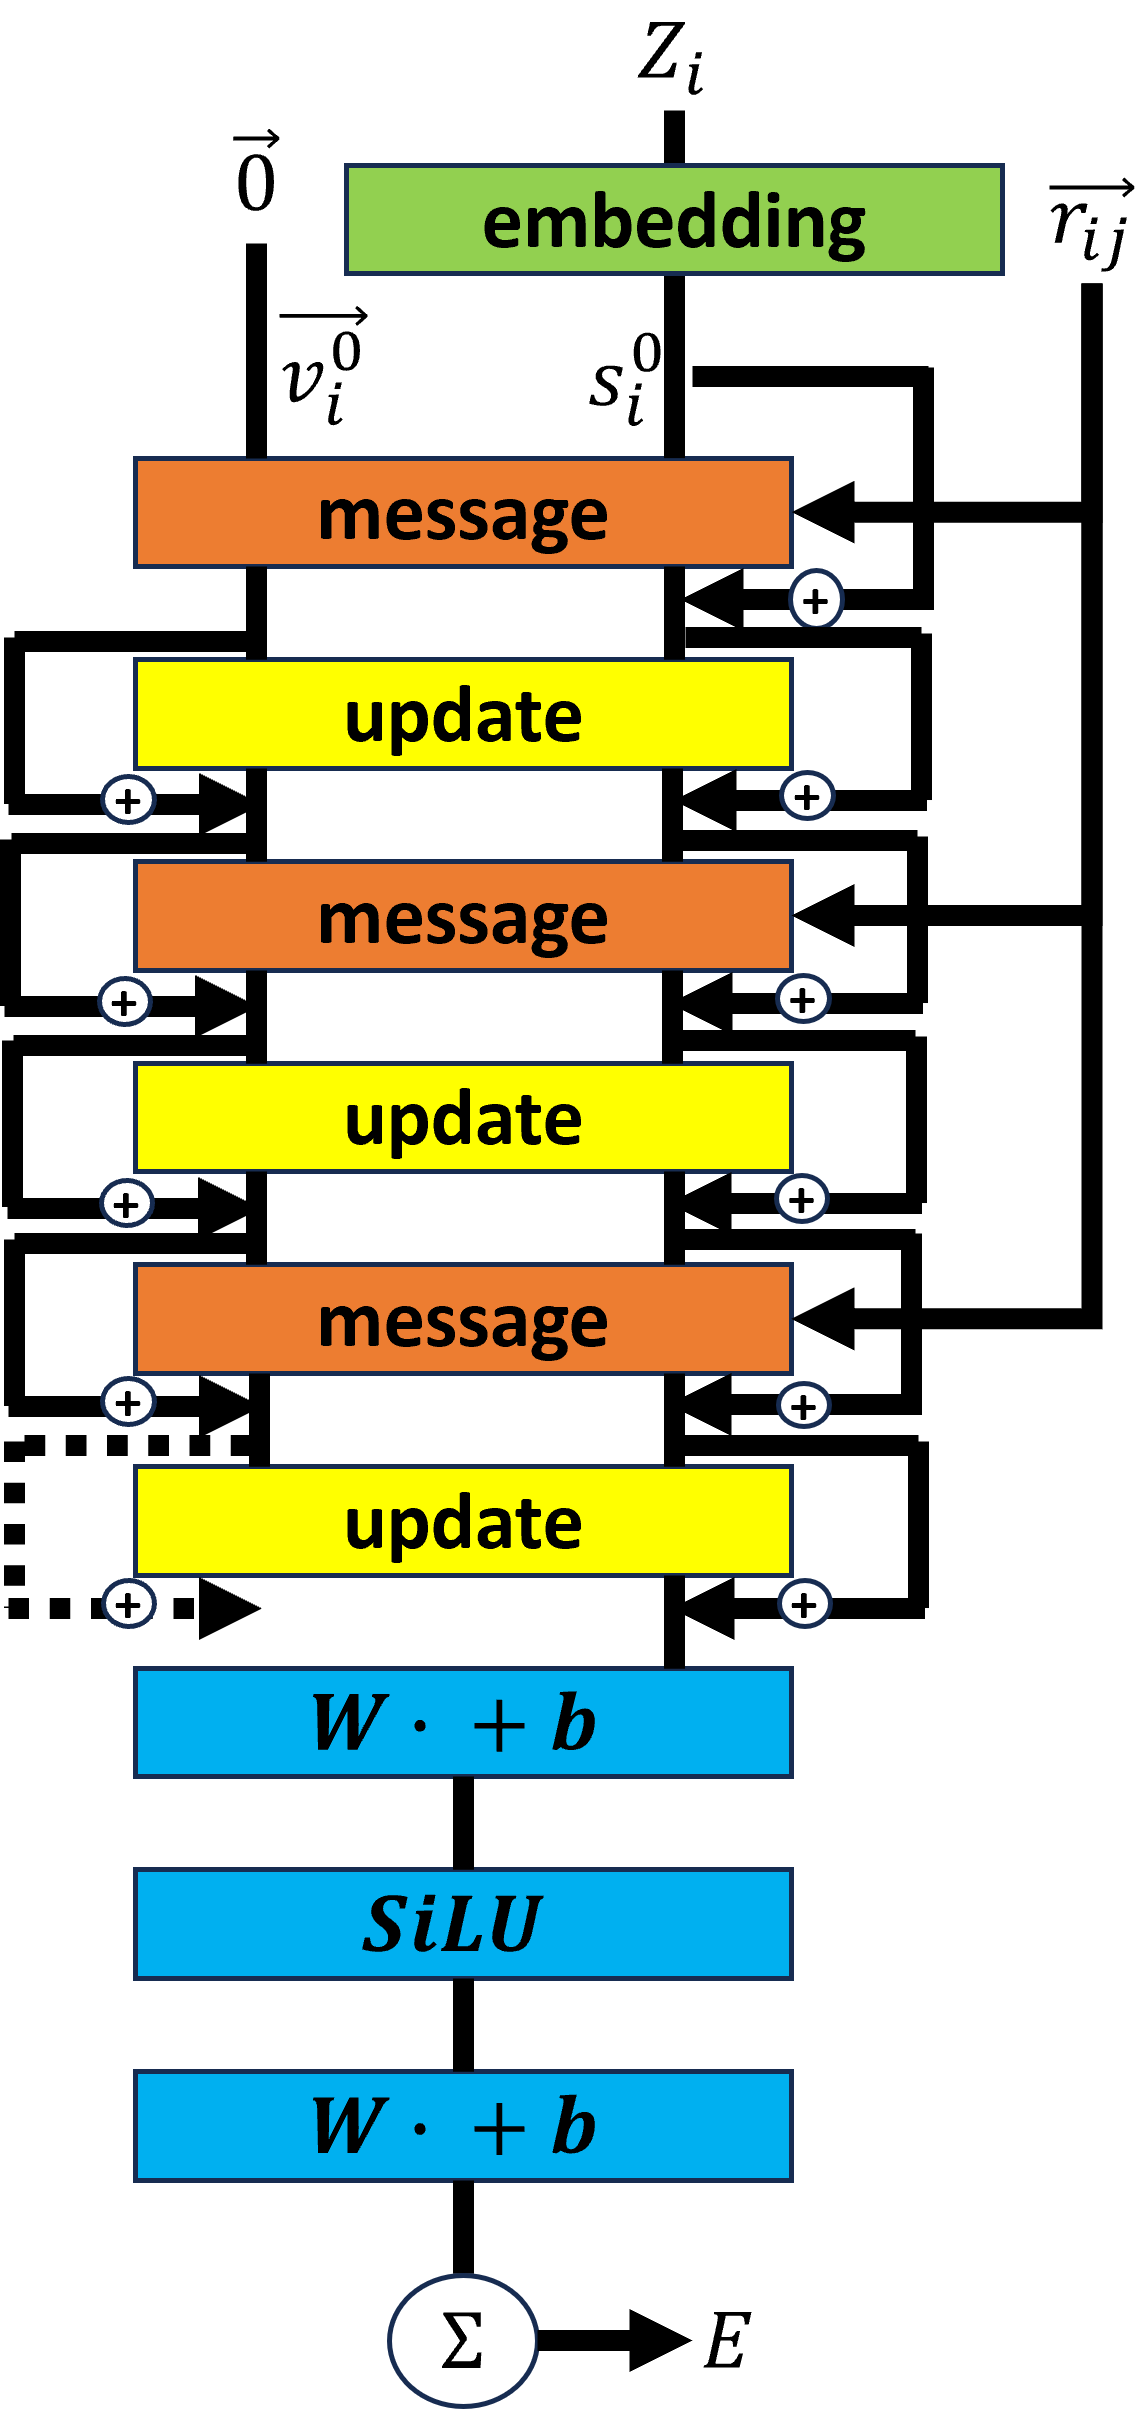
\includegraphics[width=200pt]{Images/Method/MPNN_arc.png}
\end{figure}

\subsection{Training- and Validation-loop}\label{subsec:training}

\begin{algorithm}[H]
    \begin{algorithmic}[1]
        \State Initialize size of ensemble: $T$
        \State Initialize size of batch: $B$
        \State Initialize data sets: $Td, Vd$
        \State initialize training data loader: $TD = Dataloader(B,Td)$
        \State initialize validation data loader: $VD = Dataloader(B,Vd)$
        \State Initialize number of epochs: $E$
        \State Initialize validation index: $V$

        \For {$model=1,2,\ldots, T$}

        \State Initialize MPNN model instance: $model = PAINN()$
        \State initialize MSE loss function: $loss = MSE()$
        \State Initialize Adam optimizer: $optimizer = Adam(model.parameters())$
        \State Initialize learning rate scheduler: $scheduler = StepLR(optimizer)$

        \For {$epoch=1,2,\ldots,E$}

        \For {$batch=1,2,\ldots,TD$}

        \State Normalize targets: $y = normalize(y)$
        \State Predict binding energy: $\hat{y} = model(batch)$
        \State Calculate loss: $l = loss(y,\hat{y})$
        \State Backward pass: $l.backward()$
        \State Optimizer step: $optimizer.step()$

        \If {$epoch \% V == 0$}
        \State Model in evaluation mode: $model.eval()$

        \For {$batch=1,2,\ldots,VD$}

        \State Normalize targets: $y = normalize(y)$
        \State Predict binding energy: $\hat{y} = model(batch)$
        \State Calculate loss: $l = loss(y,\hat{y})$
        \State Apply exponential smoothing: $l = l * 0.9 + l_{-1} * 0.1$
        \State Scheduler step: $scheduler.step(l)$
        \EndFor

        \EndIf
        \EndFor
        \EndFor
        \EndFor
    \end{algorithmic}
    \caption{MPNN Training Loop}
    \label{algo:MPNN_training}
\end{algorithm}

\subsection{Test Loop}\label{subsec:test}

\begin{algorithm}[H]
    \begin{algorithmic}[2]
        \State Initialize size of ensemble: $T$
        \State Initialize size of batch: $B$
        \State Initialize data sets: $Testd, $
        \State initialize training data loader: $TestD = Dataloader(B,Testd)$

        \For {$model=1,2,\ldots, T$}
        \State Initialize target list: $y_{l}$
        \State Initialize prediction list: $\hat{y}_{l}$
        \For {$batch=1,2,\ldots,TestD$}
        \State Normalize targets: $y = normalize(y)$
        \State Predict binding energy: $\hat{y} = model(batch)$
        \State Calculate loss: $l = loss(y,\hat{y})$
        \State Append target to list: $y_{l}$
        \State Append prediction to list: $\hat{y}_{l}$
        \EndFor
        \State Save predictions and targets to file
        \State Save model to file
        \EndFor
    \end{algorithmic}
    \caption{MPNN Testing Loop}
    \label{algo:MPNN_testing}
\end{algorithm}

\subsection{Modelling Hyperparameters}\label{subsec:mod-hyper}

Generally, two subsets of hyperparameters exists, those relevant to the less sophisticated set of ensemble models (titled MPNN64), and those
relevant to the more sophisticated ensemble models (titled MPNN128). The table below\ref{tab:hyperparameters},
details shared and non-shared model hyperparameters, as well
as highlighting the parameters, which are consistent with the PAINN architecture described in \cite{PAINN} with a star (*).

\begin{table}[H]
    \centering
    \caption{Modelling hyperparameters}
    \label{tab:hyperparameters}
    \begin{tabular}{|lcll|}
        \hline
        \multicolumn{1}{|l|}{\textbf{Model Hyperparameters}}                 & \multicolumn{1}{l|}{\textit{\textbf{MPNN64}}} & \multicolumn{1}{l|}{\textit{\textbf{MPNN128}}} & \textit{\textbf{Unit}} \\ \hline
        \multicolumn{4}{|c|}{\textbf{Shared}}                                                                                                                                                          \\ \hline
        \multicolumn{1}{|l|}{\textbf{Number of physical dimensions*}}        & \multicolumn{2}{c|}{3}                        & Dimensions                                                              \\ \hline
        \multicolumn{1}{|l|}{\textbf{Number of Message Passing Rounds*}}     & \multicolumn{2}{c|}{5}                        & Rounds                                                                  \\ \hline
        \multicolumn{1}{|l|}{\textbf{Patience*}}                             & \multicolumn{2}{c|}{5}                        & Validation steps                                                        \\ \hline
        \multicolumn{1}{|l|}{\textbf{Weight Decay*}}                         & \multicolumn{2}{c|}{0.01}                     & N/A                                                                     \\ \hline
        \multicolumn{1}{|l|}{\textbf{Learning Rate Decay*}}                  & \multicolumn{2}{c|}{0.5}                      & N/A                                                                     \\ \hline
        \multicolumn{1}{|l|}{\textbf{Exponential Smoothing for Validation*}} & \multicolumn{2}{c|}{0.9}                      & N/A                                                                     \\ \hline
        \multicolumn{1}{|l|}{\textbf{Radial Basis Parameter*}}               & \multicolumn{2}{c|}{20}                       & N/A                                                                     \\ \hline
        \multicolumn{1}{|l|}{\textbf{Learning Rate}}                         & \multicolumn{2}{c|}{0.001}                    & N/A                                                                     \\ \hline
        \multicolumn{1}{|l|}{\textbf{Cutoff Distance}}                       & \multicolumn{2}{c|}{4}                        & Ångstrøm                                                                \\ \hline
        \multicolumn{4}{|c|}{\textbf{Not shared}}                                                                                                                                                      \\ \hline
        \multicolumn{1}{|l|}{\textbf{State dimension size}}                  & \multicolumn{1}{c|}{64}                       & \multicolumn{1}{c|}{128}                       & Dimensions             \\ \hline
    \end{tabular}
\end{table}
%#TODO Indsæt link til appendix som forklarer de forskellige hyperparametre

An explanation of the individual hyperparameters influence on the model, and a justification for selection of the above values, can be
be found in the appendix section\ref{subsec:appendixA}.

\subsection{Experimental Hyperparameters}\label{subsec:experiement}

The experimental hyperparameters defining the implementation of the above model setting, can be found in
table below\ref{tab:experiment}.

\begin{table}[H]
    \centering
    \caption{Experimental Hyperparameters}
    \label{tab:experiment}
    \begin{tabular}{|l|c|c|}
        \hline
        \textbf{Experimental Hyperparameters}                          & \multicolumn{1}{l|}{\textit{\textbf{Value}}} & \textit{\textbf{Unit}} \\ \hline
        \multicolumn{1}{|c|}{\textbf{Number of molecules in Data Set}} & 695                                          & Molecules              \\ \hline
        \textbf{Training Split}                                        & 0.8                                          & N/A                    \\ \hline
        \textbf{Validation Split}                                      & 0.1                                          & N/A                    \\ \hline
        \textbf{Test Split}                                            & 0.1                                          & N/A                    \\ \hline
        \textbf{Ensemble Size}                                         & 5                                            & Models                 \\ \hline
        \textbf{Initial number of Epochs}                              & 200                                          & Epochs                 \\ \hline
        \textbf{Validation Index}                                      & 5                                            & Epochs                 \\ \hline
        \textbf{Model Saving Interval}                                 & 0.01                                         & N/A                    \\ \hline
        \textbf{Batch Size}                                            & 5                                            & Molecules              \\ \hline
    \end{tabular}
\end{table}

An in explanation of the selection of experiment hyperparameters and justification,
be found in the appendix section\ref{subsec:appendixB}.

\subsection{Software tools and Hardware}\label{subsec:software}

The projects execution were developed in Python 3.10.9, with heavy emphasis on Pytorch, Numpy and Pandas,
supported by few shell scripts for cloud job definitions.
A full list of packages, and their versions utilized in the experiment, can be seen in appendix\ref{subsec:appendixC}
The initial datastructures and pipeline were inspired by course-material made by Mikkel Nørgaard Schmidt.
The hardware utilized for the final experimental setup, were two two types of GPUs, belonging
to the High Performance Computing (HPC) cluster at the Technical University of Denmark (DTU).
The two queues utilized were 'gpua100' and 'gpuv100'. For further details on the hardware,
please refer to the following reference:\cite{hpc}. Total computation time in the cloud was three days,
in order to produce the trained ensemble of ten individual models.

\subsection{Reproduceability}\label{subsec:reproduceability}

For reviewing and reproduceability purposes,
the following github link stores the latest version of the code: \url{https://github.com/Lohmann94/head},
which was utilized in the experiment. The experiment can be reproduced with the following seed-values\ref{tab:seeds},
which can be found for individual models:

\begin{table}[H]
    \centering
    \caption{Model seeds for reproduction}
    \label{tab:seeds}
    \begin{tabular}{|cc|cc|}
        \hline
        \multicolumn{2}{|c|}{\textbf{MPNN128 Ensemble:}} & \multicolumn{2}{c|}{\textbf{MPNN64 Ensemble:}}                                                                         \\ \hline
        \multicolumn{1}{|c|}{\textit{\textbf{Model}}}    & \textit{\textbf{Seed}}                         & \multicolumn{1}{c|}{\textit{\textbf{Model}}} & \textit{\textbf{Seed}} \\ \hline
        \multicolumn{1}{|c|}{\textbf{MPNN128\_1}}        & 49                                             & \multicolumn{1}{c|}{\textbf{MPNN64\_1}}      & 90                     \\ \hline
        \multicolumn{1}{|c|}{\textbf{MPNN128\_2}}        & 10                                             & \multicolumn{1}{c|}{\textbf{MPNN64\_2}}      & 52                     \\ \hline
        \multicolumn{1}{|c|}{\textbf{MPNN128\_3}}        & 100                                            & \multicolumn{1}{c|}{\textbf{MPNN64\_3}}      & 7                      \\ \hline
        \multicolumn{1}{|c|}{\textbf{MPNN128\_4}}        & 20                                             & \multicolumn{1}{c|}{\textbf{MPNN64\_4}}      & 9                      \\ \hline
        \multicolumn{1}{|c|}{\textbf{MPNN128\_5}}        & 30                                             & \multicolumn{1}{c|}{\textbf{MPNN64\_5}}      & 87                     \\ \hline
    \end{tabular}
\end{table}

The cloud-job configuration variables for reproducing with the described performance,
can be found in the below table\ref{tab:cloud-job-param}:

\begin{table}[]
    \centering
    \caption{Cloud Job Parameters}
    \label{tab:cloud-job-param}
    \begin{tabular}{|c|c|c|}
        \hline
        \textbf{Cloud Job Parameters} & \textit{\textbf{MPNN128}} & \textit{\textbf{MPNN64}}              \\ \hline
        \textbf{Queue}                & \textbf{gpuv100}          & \multicolumn{1}{l|}{\textbf{gpua100}} \\ \hline
        \textbf{Number of cores}      & 8                         & 8                                     \\ \hline
        \textbf{Memory/Cores}         & 5 gb                      & 5 gb                                  \\ \hline
        \textbf{Number of hosts}      & 1                         & 1                                     \\ \hline
    \end{tabular}
\end{table}

\newpage
